\documentclass[conference]{IEEEtran}
% \IEEEoverridecommandlockouts
% The preceding line is only needed to identify funding in the first footnote. If that is unneeded, please comment it out.
\usepackage{cite}
\usepackage{amsmath,amssymb,amsfonts}
\usepackage{algorithmic}
\usepackage{graphicx}
\usepackage{textcomp}
\usepackage{xcolor}
\usepackage{hyperref}
\usepackage{float}
\usepackage[portuguese]{babel}

\addto\captionsportuguese{\renewcommand{\figurename}{Fig.}}
\addto\captionsportuguese{\renewcommand{\tablename}{TABELA}}

\def\BibTeX{{\rm B\kern-.05em{\sc i\kern-.025em b}\kern-.08em
    T\kern-.1667em\lower.7ex\hbox{E}\kern-.125emX}}
\begin{document}

%\title{Conference Paper Title*\\
%{\footnotesize \textsuperscript{*}Note: Sub-titles are not captured in Xplore and
%should not be used}
%\thanks{Identify applicable funding agency here. If none, delete this.}
%}

\title{ \LARGE \MakeUppercase{Método de aprimoramento de processamentos de imagens aplicados à detecção e classificação de falhas em cadeias de isoladores}}


\author{
\renewcommand{\arraystretch}{0.9}%
\makebox[\textwidth]{%
\hfill
\begin{tabular}[t]{@{}c@{}}
{\large1\textsuperscript{st} Luan Willig Silveira}\\
{\normalsize\textit{Engenharia Elétrica}}\\
{\normalsize\textit{Universidade Federal de Santa Maria}}\\
{\normalsize Cachoeira do Sul, Brasil}\\
{\normalsize luan.w.silveira@gmail.com}
\end{tabular}%
\hfill
\begin{tabular}[t]{@{}c@{}}
{\large2\textsuperscript{nd} Paulo César Vargas Luz}\\
{\normalsize\textit{Engenharia Elétrica}}\\
{\normalsize\textit{Universidade Federal de Santa Maria}}\\
{\normalsize Cachoeira do Sul, Brasil}\\
{\normalsize paulo.c.luz@ufsm.br}
\end{tabular}%
\hfill
\begin{tabular}[t]{@{}c@{}}
{\large3\textsuperscript{rd} Daniel Pinheiro Bernardon}\\
{\normalsize\textit{Engenharia Elétrica}}\\
{\normalsize\textit{Universidade Federal de Santa Maria}}\\
{\normalsize Santa Maria, Brasil}\\
{\normalsize dpbernardon@ufsm.br}
\end{tabular}%
\hfill}%
\\[1.8em]
\makebox[\textwidth]{%
\hfill
\begin{tabular}[t]{@{}c@{}}
{\large4\textsuperscript{th} Dion Lenon Prediger Feil}\\
{\normalsize\textit{Engenharia Elétrica}}\\
{\normalsize\textit{Universidade Federal de Santa Maria}}\\
{\normalsize Cachoeira do Sul, Brasil}\\
{\normalsize dion.feil@ufsm.br}
\end{tabular}%
\hfill
\begin{tabular}[t]{@{}c@{}}
{\large5\textsuperscript{th} Laura Lisiane Callai dos Santos}\\
{\normalsize\textit{Engenharia Elétrica}}\\
{\normalsize\textit{Universidade Federal de Santa Maria}}\\
{\normalsize Cachoeira do Sul, Brasil}\\
{\normalsize laura.santos@ufsm.br}
\end{tabular}%
\hfill
\begin{tabular}[t]{@{}c@{}}
{\large6\textsuperscript{th} Nelson Knak Neto}\\
{\normalsize\textit{Engenharia Elétrica}}\\
{\normalsize\textit{Universidade Federal de Santa Maria}}\\
{\normalsize Cachoeira do Sul, Brasil}\\
{\normalsize nelson.knak@ufsm.br}
\end{tabular}%
\hfill}%
}

\maketitle

\begin{abstract}
A crescente demanda por sistemas automatizados de inspeção de linhas de transmissão de energia elétrica utilizando visão computacional impulsiona o uso de inteligência artificial. No entanto, não há uma metodologia padronizada para definir estratégias de processamento e seus ajustes paramétricos que permita uma comparação real de desempenho. Este trabalho propõe uma metodologia sistemática para comparar, selecionar e aprimorar técnicas de processamento de imagens, visando otimizar o desempenho preditivo de Redes Neurais Convolucionais (CNNs) na detecção de falhas. Utilizando os \textit{datasets} CPLID e DRNPW, constatou-se que o efeito do pré-processamento depende do cenário de captura. Em imagens de fundo homogêneo (CPLID), o ganho simples de contraste (\textit{Contrast Enhancement}) alcançou 95,35\% de acurácia, contra 93,02\% da imagem sem tratamento, diferença de um acerto em 43 imagens de teste, ao passo que o desfoque gaussiano derrubou o desempenho para 67,44\%. Já em imagens obtidas por drones sobre fundos poluídos (DRNPW), combinar realce de contraste e equalização de histograma elevou a acurácia de 63,33\% para 83,33\%, seis acertos em 30 imagens. A otimização paramétrica via busca em grade (\textit{Grid Search}) confirmou um fator ideal de ajuste de contraste situado em torno de 1,33, mitigando interferências destrutivas. Os resultados comprovam que não há uma técnica universalmente superior, dependendo substancialmente das características intrínsecas da imagem e do ambiente de captura. Dessa forma, a metodologia proposta viabiliza uma comparação justa e reprodutível entre as diversas técnicas de processamento de imagens, oferecendo um caminho sistemático para a seleção e o aprimoramento de estratégias de pré-processamento voltadas à detecção automatizada de falhas em cadeias de isoladores.
\end{abstract}

\begin{IEEEkeywords}
processamento de imagens, redes neurais convolucionais, cadeias de isoladores, detecção de falhas, inteligência artificial
\end{IEEEkeywords}


\section{Introdução}

A crescente demanda por sistemas automatizados de inspeção de cadeias de isoladores evidencia a necessidade de técnicas avançadas de processamento de imagem para a detecção precoce de falhas. A análise digital de imagens permite extrair características relevantes para identificar anomalias em componentes elétricos, possibilitando diagnósticos mais precisos nas linhas de transmissão de energia \cite{Gonzalez2008}. 

Ademais, o emprego de redes neurais, e mais especificamente as Redes Neurais Convolucionais (CNNs), tem se destacado na resolução de problemas complexos de classificação e detecção, contribuindo para a robustez dos sistemas de inspeção \cite{LeCun2015, Krizhevsky2012}. Contudo, a eficácia preditiva desses modelos de inteligência artificial depende intrinsecamente da qualidade das imagens de entrada. Revisões dedicadas ao tema em outros domínios de análise de imagens mostram que a escolha das etapas de pré-processamento altera de forma mensurável o desempenho final dos modelos \cite{Salvi2021}, e que os parâmetros que controlam essas etapas podem ser ajustados por métodos sistemáticos de busca, como a busca em grade e a busca aleatória \cite{yang2020hyperparameter}.

Assim, o presente estudo tem como objetivo desenvolver uma metodologia escalável capaz de comparar, selecionar, combinar e aprimorar técnicas de processamento de imagem para a detecção e classificação de falhas em cadeias de isoladores elétricos. Para isso, são estabelecidas métricas quantitativas de acurácia e \textit{F1-score}, bem como avaliadas estratégias unificadas e compostas de tratamentos de imagem aplicadas em dois conjuntos de dados distintos da área (CPLID e DRNPW).

\section{Fundamentação Teórica e Trabalhos Relacionados}

A utilização de ferramentas de inteligência artificial para diagnósticos em equipamentos tem se destacado como uma solução promissora no contexto da manutenção preventiva, especialmente diante do aumento da complexidade dos sistemas industriais do setor elétrico e da necessidade de maior confiabilidade operacional \cite{nguyen2018automatic}. A detecção precoce de falhas em componentes como cadeias de isoladores, transformadores e suportes de linhas de transmissão é fundamental para evitar interrupções de longo prazo e reduzir custos associados à intervenção humana direta \cite{wang2023, eze2022deep}.

\subsection{Processamento de Imagens e Redes Neurais}

O processamento de imagens tem papel fundamental na preparação dos dados visuais antes de sua entrada em redes profundas. Imagens capturadas por Veículos Aéreos Não Tripulados (VANTs) ou câmeras de inspeção frequentemente apresentam ruídos, interferência climática, variações fortes de iluminação e fundos com vegetação e poluição ambiental, condições apontadas como um dos principais obstáculos à inspeção visual automatizada de linhas de transmissão \cite{nguyen2018automatic}.

Entre as técnicas fundamentais destacam-se a normalização e a padronização de histogramas, aplicadas para reduzir variações bruscas de intensidade luminosa nos canais RGB, o que facilita a convergência durante o treinamento das redes \cite{sharma2024deep, chen2023robustness}. Da mesma forma, o redimensionamento padronizado reduz o custo computacional e adequa as imagens ao tamanho de entrada exigido pela primeira camada convolucional, enquanto o aumento de dados (\textit{Data Augmentation}) compensa a escassez de falhas reais catalogadas, gerando variações sintéticas que melhoram a robustez do classificador \cite{shorten2019survey}.

O ajuste de contraste é especialmente crítico no contexto de isoladores. Enquanto a \textit{Contrast Limited Adaptive Histogram Equalization} (CLAHE) evita a amplificação excessiva de ruído ao subdividir a imagem para correção localizada \cite{pizer1987adaptive}, a equalização global favorece a separação nítida das bordas do material cerâmico ou vítreo deteriorado. Contudo, intervenções muito agressivas, como filtros de supressão excessivos, podem eliminar texturas importantes que caracterizam pequenas fraturas ou contaminações na superfície do equipamento \cite{ozturk2018histopathological}.

Esse cuidado com o tratamento inicial reflete-se diretamente no desempenho das Redes Neurais Convolucionais (CNNs). Diferentemente das redes \textit{Feed-Forward} tradicionais, as CNNs preservam a estrutura espacial da imagem por meio de convoluções com \textit{kernels} locais, reduzem a dimensionalidade via \textit{MaxPooling} e extraem mapas hierárquicos de textura e contraste \cite{LeCun2015}. Entretanto, sua capacidade de identificar anomalias na rede elétrica depende diretamente da representatividade dos dados, o que reforça a importância do tratamento da imagem de entrada, conforme a estrutura ilustrada na Fig. \ref{fig:cnn}.

\begin{figure}[H]
    \centering
    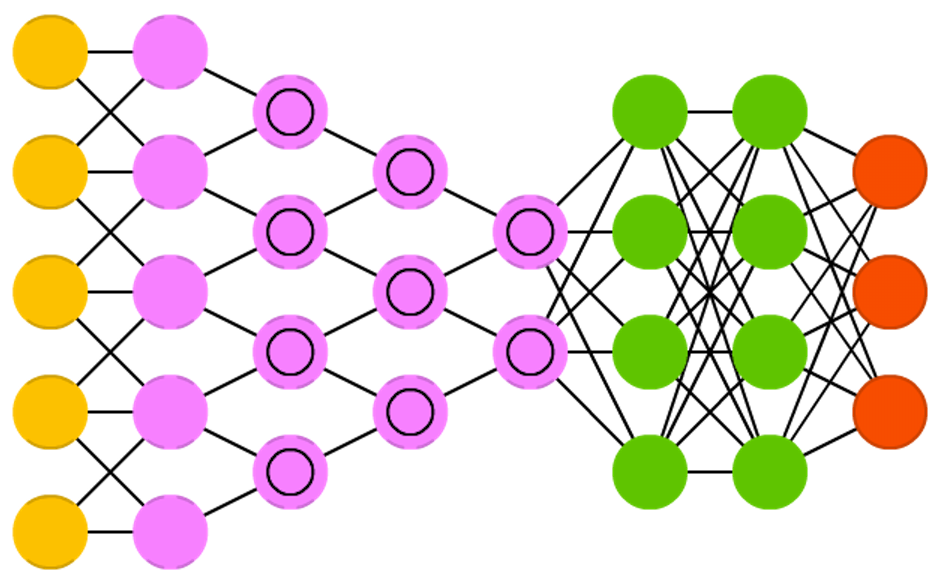
\includegraphics[width=0.42\textwidth]{img/cnn.png}
    \caption{Representação estrutural típica de uma Rede Neural Convolucional na extração de características visuais.}
    \label{fig:cnn}
\end{figure}

\subsection{Trabalhos Correlatos e Lacunas da Literatura}

Os trabalhos que avaliam o efeito do pré-processamento sobre modelos convolucionais não convergem para uma conclusão única. Revisões da área registram que a integração de etapas de pré-processamento ao fluxo de aprendizado profundo costuma elevar o desempenho em relação à rede isolada \cite{Salvi2021, sciencedirect2023normalization}. Estudos comparativos controlados, porém, encontram o resultado oposto em determinados conjuntos, com desempenho superior sobre as imagens sem tratamento \cite{rodrigues2020comparing, ozturk2018histopathological}.

Por um lado, diversos estudos relatam ganhos expressivos de acurácia a partir de pré-processamentos elaborados. Por exemplo, uma abordagem que encadeia a localização do isolador por Faster RCNN, a remoção do fundo por segmentação e a descrição morfológica do defeito sobre a imagem binarizada relatou \textit{recall} de 0,98 na localização dos isoladores e acurácia de 0,98 na identificação do defeito, em imagens com fundo complexo \cite{zhang2022}. De forma semelhante, arquiteturas baseadas no \textit{framework} YOLO (YOLOv7) mostraram-se eficientes para detectar pequenos defeitos na isolação quando aliadas a ajustes de arquitetura voltados a mecanismos de atenção \cite{zheng2022improved}.

Em contrapartida, há pesquisas que questionam a intervenção excessiva sobre a imagem. Ao comparar seis estratégias de pré-processamento e cinco arquiteturas convolucionais na classificação de células HEp-2 em imagens de imunofluorescência, cujo comparativo é ilustrado na Fig. \ref{fig:preprocessing_rodrigues}, o melhor resultado, 98,28\% de acurácia, foi obtido com a rede Inception-V3 treinada do zero sobre imagens sem pré-processamento e com aumento de dados \cite{rodrigues2020comparing}.

\begin{figure}[H]
    \centering
    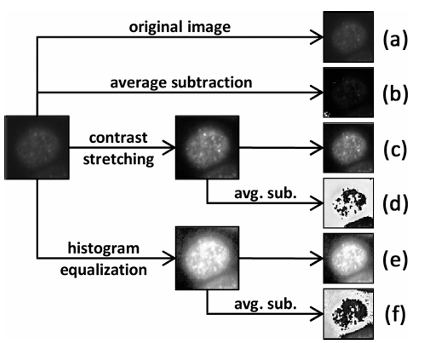
\includegraphics[width=0.44\textwidth]{img/preprocessing_rodrigues2020comparing.png}
    \caption{Comparativo de estratégias de processamento de imagens propostas na literatura para avaliação de modelos preditivos \cite{rodrigues2020comparing}.}
    \label{fig:preprocessing_rodrigues}
\end{figure}

Essa perspectiva é reforçada por trabalhos que comparam níveis crescentes de tratamento e observam queda de desempenho no grupo de sobre-processamento, em que a limiarização e as operações morfológicas somadas ao realce removem justamente as características que a rede seria capaz de aprender sozinha \cite{ozturk2018histopathological}. No domínio da inspeção elétrica, parte dos trabalhos concentra o esforço na arquitetura do detector em vez do tratamento prévio da imagem, como no modelo CSPD-YOLO, aplicado diretamente a imagens aéreas de fundo complexo \cite{liu2021}, e na rede convolucional com atenção recursiva RA-CNN, avaliada sobre imagens de isoladores em condições atmosféricas adversas \cite{wang2023}.

Essa divergência expõe uma lacuna importante: a falta de um método para determinar o limite adequado de realce em diferentes tipos de imagem. Os trabalhos raramente exploram de forma quantitativa o efeito isolado do fator de correção, adotando configurações fixas. O presente trabalho, conforme detalhado nas próximas seções, busca preencher essa lacuna ao avaliar sistematicamente esse parâmetro por meio de \textit{Grid Search} sobre o ganho de contraste, oferecendo uma referência prática sobre quando e quanto uma imagem de inspeção deve ser processada.

\section{Metodologia}
\label{sec:metodologia}

A metodologia proposta segue um fluxo estruturado para otimizar o processamento aplicado às imagens de entrada de uma CNN. O processo geral, detalhado na Fig. \ref{fig:metodologia_geral}, envolve, de forma iterativa, a seleção de \textit{datasets}, o pré-processamento da imagem, o ajuste paramétrico e a avaliação por meio do treinamento dos modelos.

\begin{figure}[H]
    \centering
    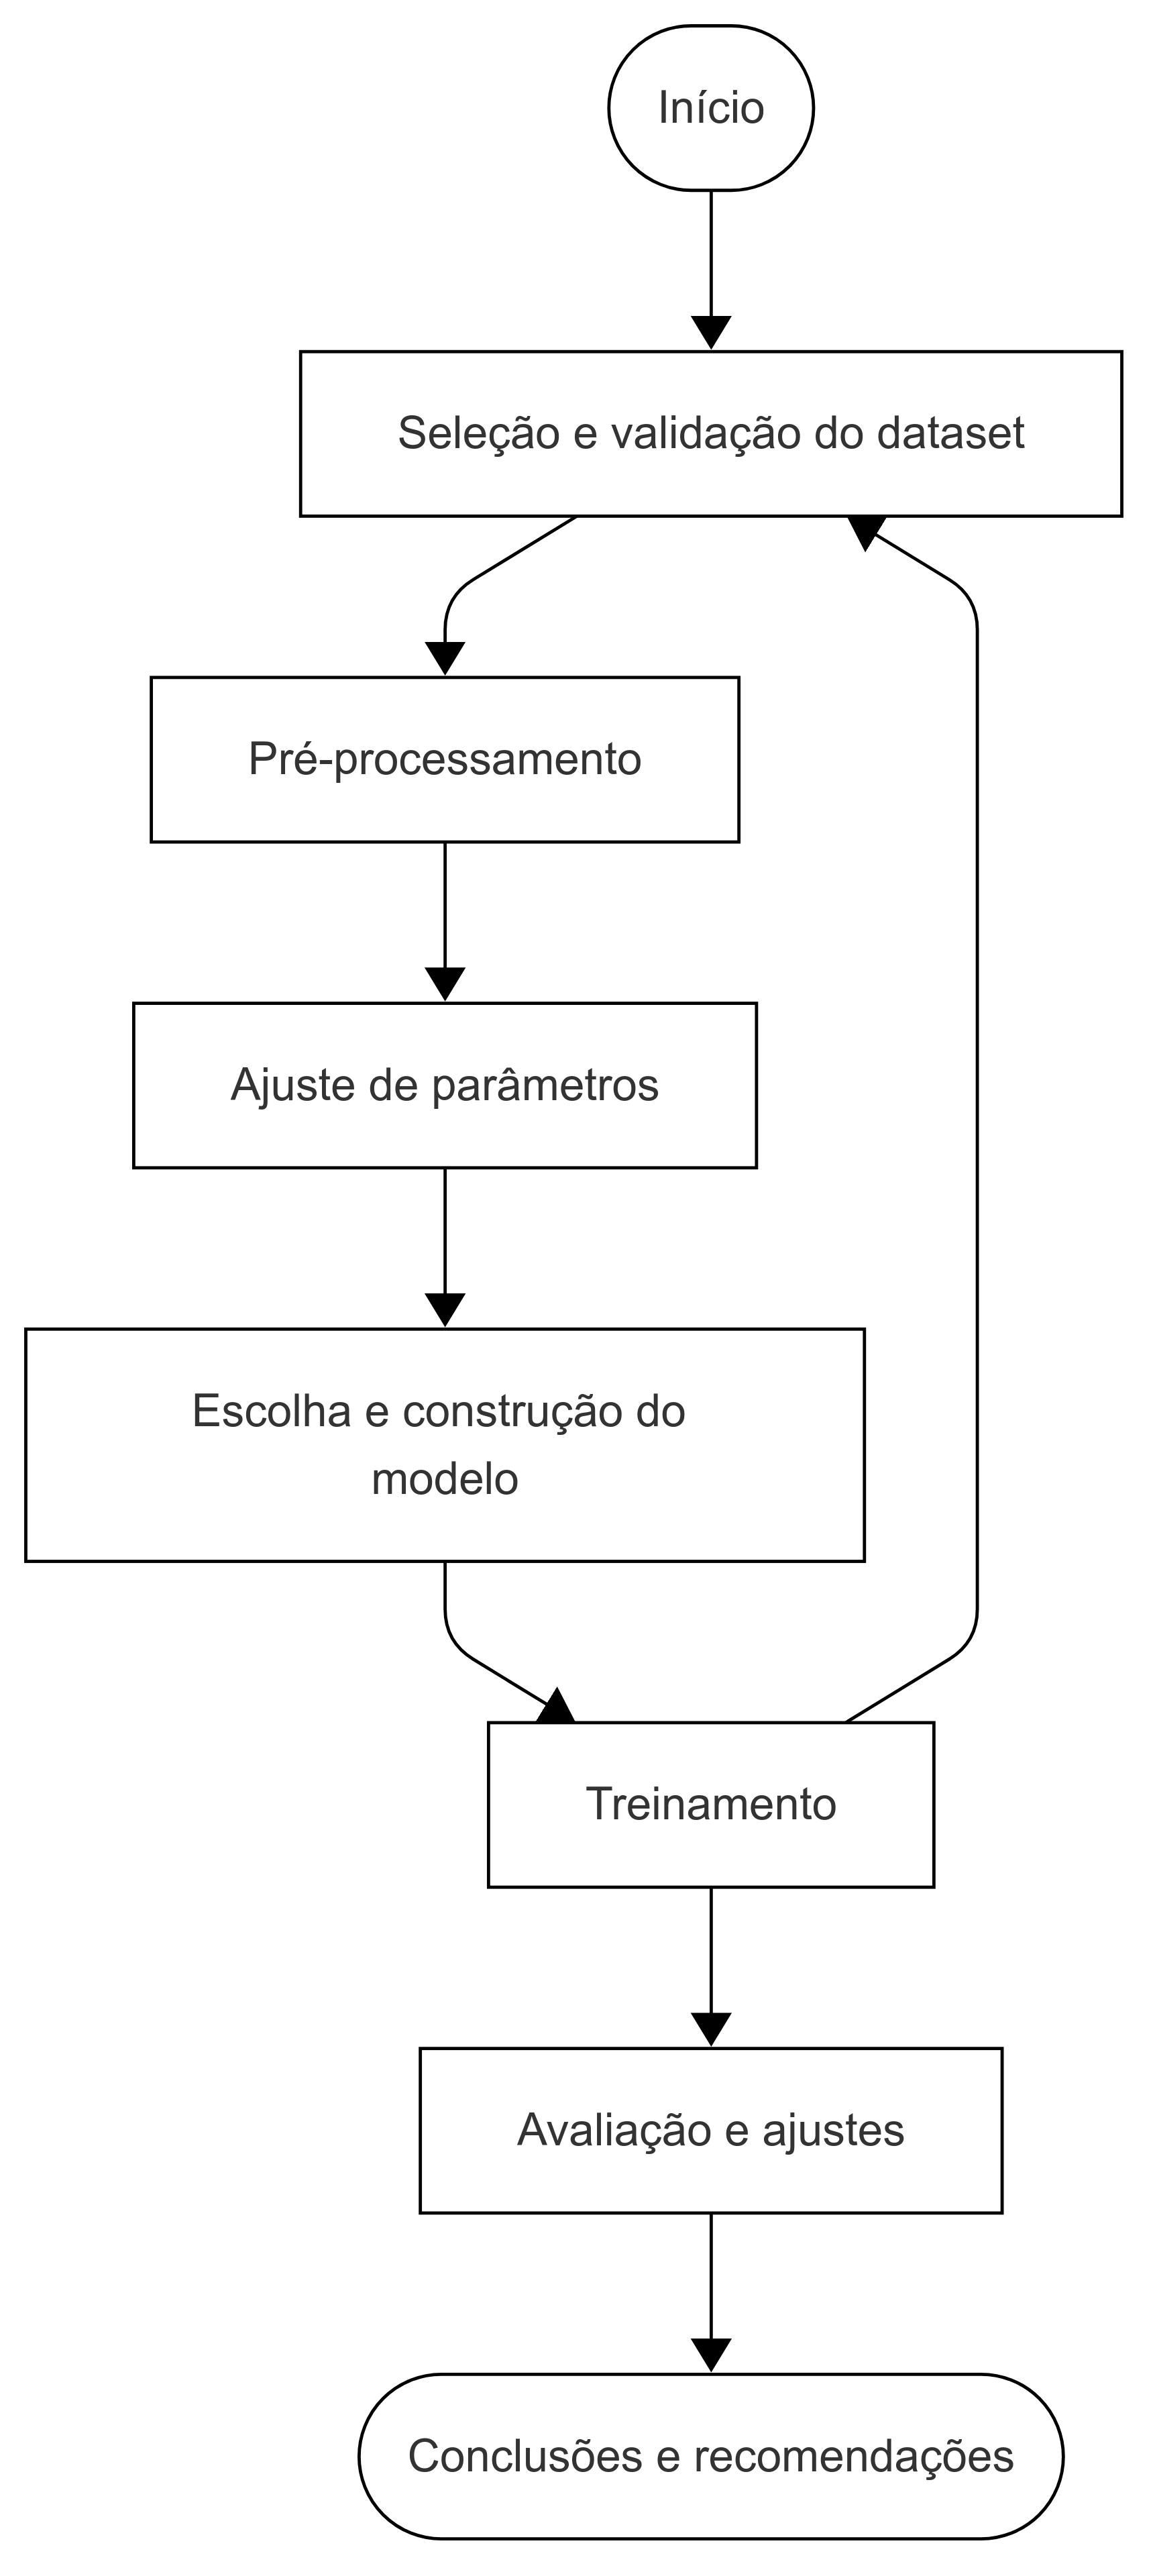
\includegraphics[width=0.30\textwidth]{img/metodologia - geral.png}
    \caption{Fluxograma geral da metodologia proposta, detalhando o processo iterativo de tratamento e avaliação.}
    \label{fig:metodologia_geral}
\end{figure}

A qualidade, a quantidade e a diversidade dos dados exercem um impacto direto no treinamento das redes profundas \cite{shorten2019survey, he2009learning}. Por esta razão, empregaram-se dois importantes conjuntos de dados de imagens no estudo:
\begin{enumerate}
    \item \textbf{CPLID (\textit{Chinese Power Line Insulator Dataset}):} Base caracterizada por fundos homogêneos, com recortes de isoladores sadios e com fraturas visíveis nas peças de vidro ou cerâmica.
    \item \textbf{DRNPW (\textit{Dataset for Recognition of Non-ceramic Pollution on Windings}):} Composto por recortes obtidos em inspeção aérea com drones. As amostras possuem fundos ruidosos, com forte presença de componentes adjacentes e vegetação.
\end{enumerate}

Cada conjunto foi particionado uma única vez em treinamento, validação e teste, e a mesma partição foi reutilizada em todas as variantes de pré-processamento, de modo que a única variável entre os experimentos fosse o tratamento aplicado à imagem. O CPLID divide-se em 678 imagens de treino, 127 de validação e 43 de teste, em 2 classes. O DRNPW divide-se em 468, 87 e 30 imagens, em 70 categorias declaradas, das quais apenas 59 aparecem no treino, com 335 das 468 imagens de treino em uma única categoria, o que caracteriza um desbalanceamento acentuado. As métricas relatadas na avaliação dos pré-processamentos referem-se ao conjunto de teste.

Para validar os processamentos, adotou-se a mesma arquitetura de CNN em todas as avaliações, implementada em TensorFlow/Keras. A rede recebe tensores RGB de $512 \times 512$ pixels no CPLID e de $640 \times 640$ pixels no DRNPW, e é composta por duas camadas convolucionais com 32 filtros de $3 \times 3$ e ativação ReLU, cada uma seguida de \textit{Max-Pooling} com janela de $4 \times 4$, uma camada de achatamento (\textit{Flatten}), uma camada densa com 8 unidades e ativação ReLU e uma camada de saída com ativação \textit{Softmax}, dimensionada conforme o número de rótulos do conjunto. O treinamento usou o otimizador Adam, a função de perda de entropia cruzada categórica esparsa e 50 épocas, com aumento de dados em tempo de treino por rotações, translações e inversões. A escolha de uma rede deliberadamente simples é intencional, pois, com poucos parâmetros livres, a variação observada entre os experimentos pode ser atribuída ao pré-processamento, e não à capacidade do modelo.

Na etapa de \textbf{Pré-processamento}, os filtros descritos na Seção IV-A foram testados de forma isolada e combinada. A técnica de \textit{Contrast Enhancement} recebe destaque por ajustar o contraste global dos canais RGB por meio de um fator configurável.

Por fim, após identificar a configuração de melhor desempenho, realizou-se uma etapa de \textbf{Ajuste Paramétrico} com busca em grade (\textit{Grid Search}), a fim de encontrar o valor ideal do hiperparâmetro de contraste (variável \texttt{factor}) \cite{yang2020hyperparameter}.

\section{Resultados e Discussões}

\subsection{Delineamento dos Experimentos e Arquitetura}

Os experimentos submeteram a rede descrita na Seção \ref{sec:metodologia} a 14 grupos distintos de pré-processamento nas bases CPLID e DRNPW. O grupo de controle usou as imagens originais (\textit{Original Image}). Foram testados a limiarização (\textit{Adaptive Threshold}), a detecção de contornos (\textit{Edge Detection}), a conversão para tons de cinza (\textit{Gray Scale}) e a supressão de ruído (\textit{Gaussian Blur}, \textit{Median Blur} e \textit{Fast NL-Means Denoise}). O foco principal esteve nas abordagens de iluminação, com equalizações de histograma adaptativas (CLAHE) e globais (\textit{Equalize Histogram}) e métodos de ganho direto (\textit{Contrast Enhancement}), aplicados isoladamente e em combinações híbridas, para avaliar o limite do processamento sequencial.

Como os dois conjuntos de teste são desbalanceados, adota-se o piso majoritário como referência de leitura dos valores absolutos, definido como a acurácia de responder sempre a classe mais frequente, sem observar a imagem. Ele é de 74,42\% no CPLID, onde 32 das 43 imagens de teste são \textit{Normal Insulators}, e de 73,33\% no DRNPW, onde 22 das 30 imagens pertencem a uma única categoria. Resultados abaixo desses valores indicam que o modelo não extraiu informação útil das imagens. Vale registrar ainda que, com conjuntos desse tamanho, cada acerto equivale a 2,33 pontos percentuais no CPLID e a 3,33 pontos no DRNPW. Nesse enquadramento, os testes mostraram que a eficácia de cada técnica depende fortemente do tipo de fundo presente na imagem.

\subsection{Avaliação no \textit{Dataset} CPLID}

Devido ao fundo predominantemente homogêneo dessas imagens, as técnicas baseadas no realce direto da iluminação apresentaram os melhores resultados do conjunto. O uso isolado do filtro \textbf{\textit{Contrast Enhancement}} alcançou 95,35\% de acurácia e 96,55\% de \textit{F1-score}. Combinações de \textit{Contrast Enhancement} com equalização adaptativa obtiveram valores de acurácia equivalentes.

Cabe, contudo, uma ressalva sobre a magnitude desse ganho. A amostra de controle, sem qualquer tratamento, já alcança 93,02\%, de modo que a diferença para o melhor pré-processamento é de 41 acertos contra 40, em 43 imagens. Uma única imagem separa as duas condições, dentro da flutuação esperada para um conjunto desse tamanho, o que não sustenta, isoladamente, a superioridade do realce de contraste sobre a imagem original neste cenário.

O efeito no sentido oposto, esse sim, aparece com clareza. Filtros de desfoque, em especial o \textbf{\textit{Gaussian Blur}}, atenuaram as bordas das anomalias e levaram o desempenho a 67,44\%, 25,58 pontos abaixo da imagem original e abaixo do próprio piso majoritário. Em fundos homogêneos, portanto, o pré-processamento tem margem estreita para ajudar e ampla para prejudicar, e a utilidade prática da metodologia está em descartar as transformações destrutivas antes do treinamento. O desempenho das 14 variações testadas é apresentado na Fig. \ref{fig:cplid_acc}.

\begin{figure}[H]
    \centering
    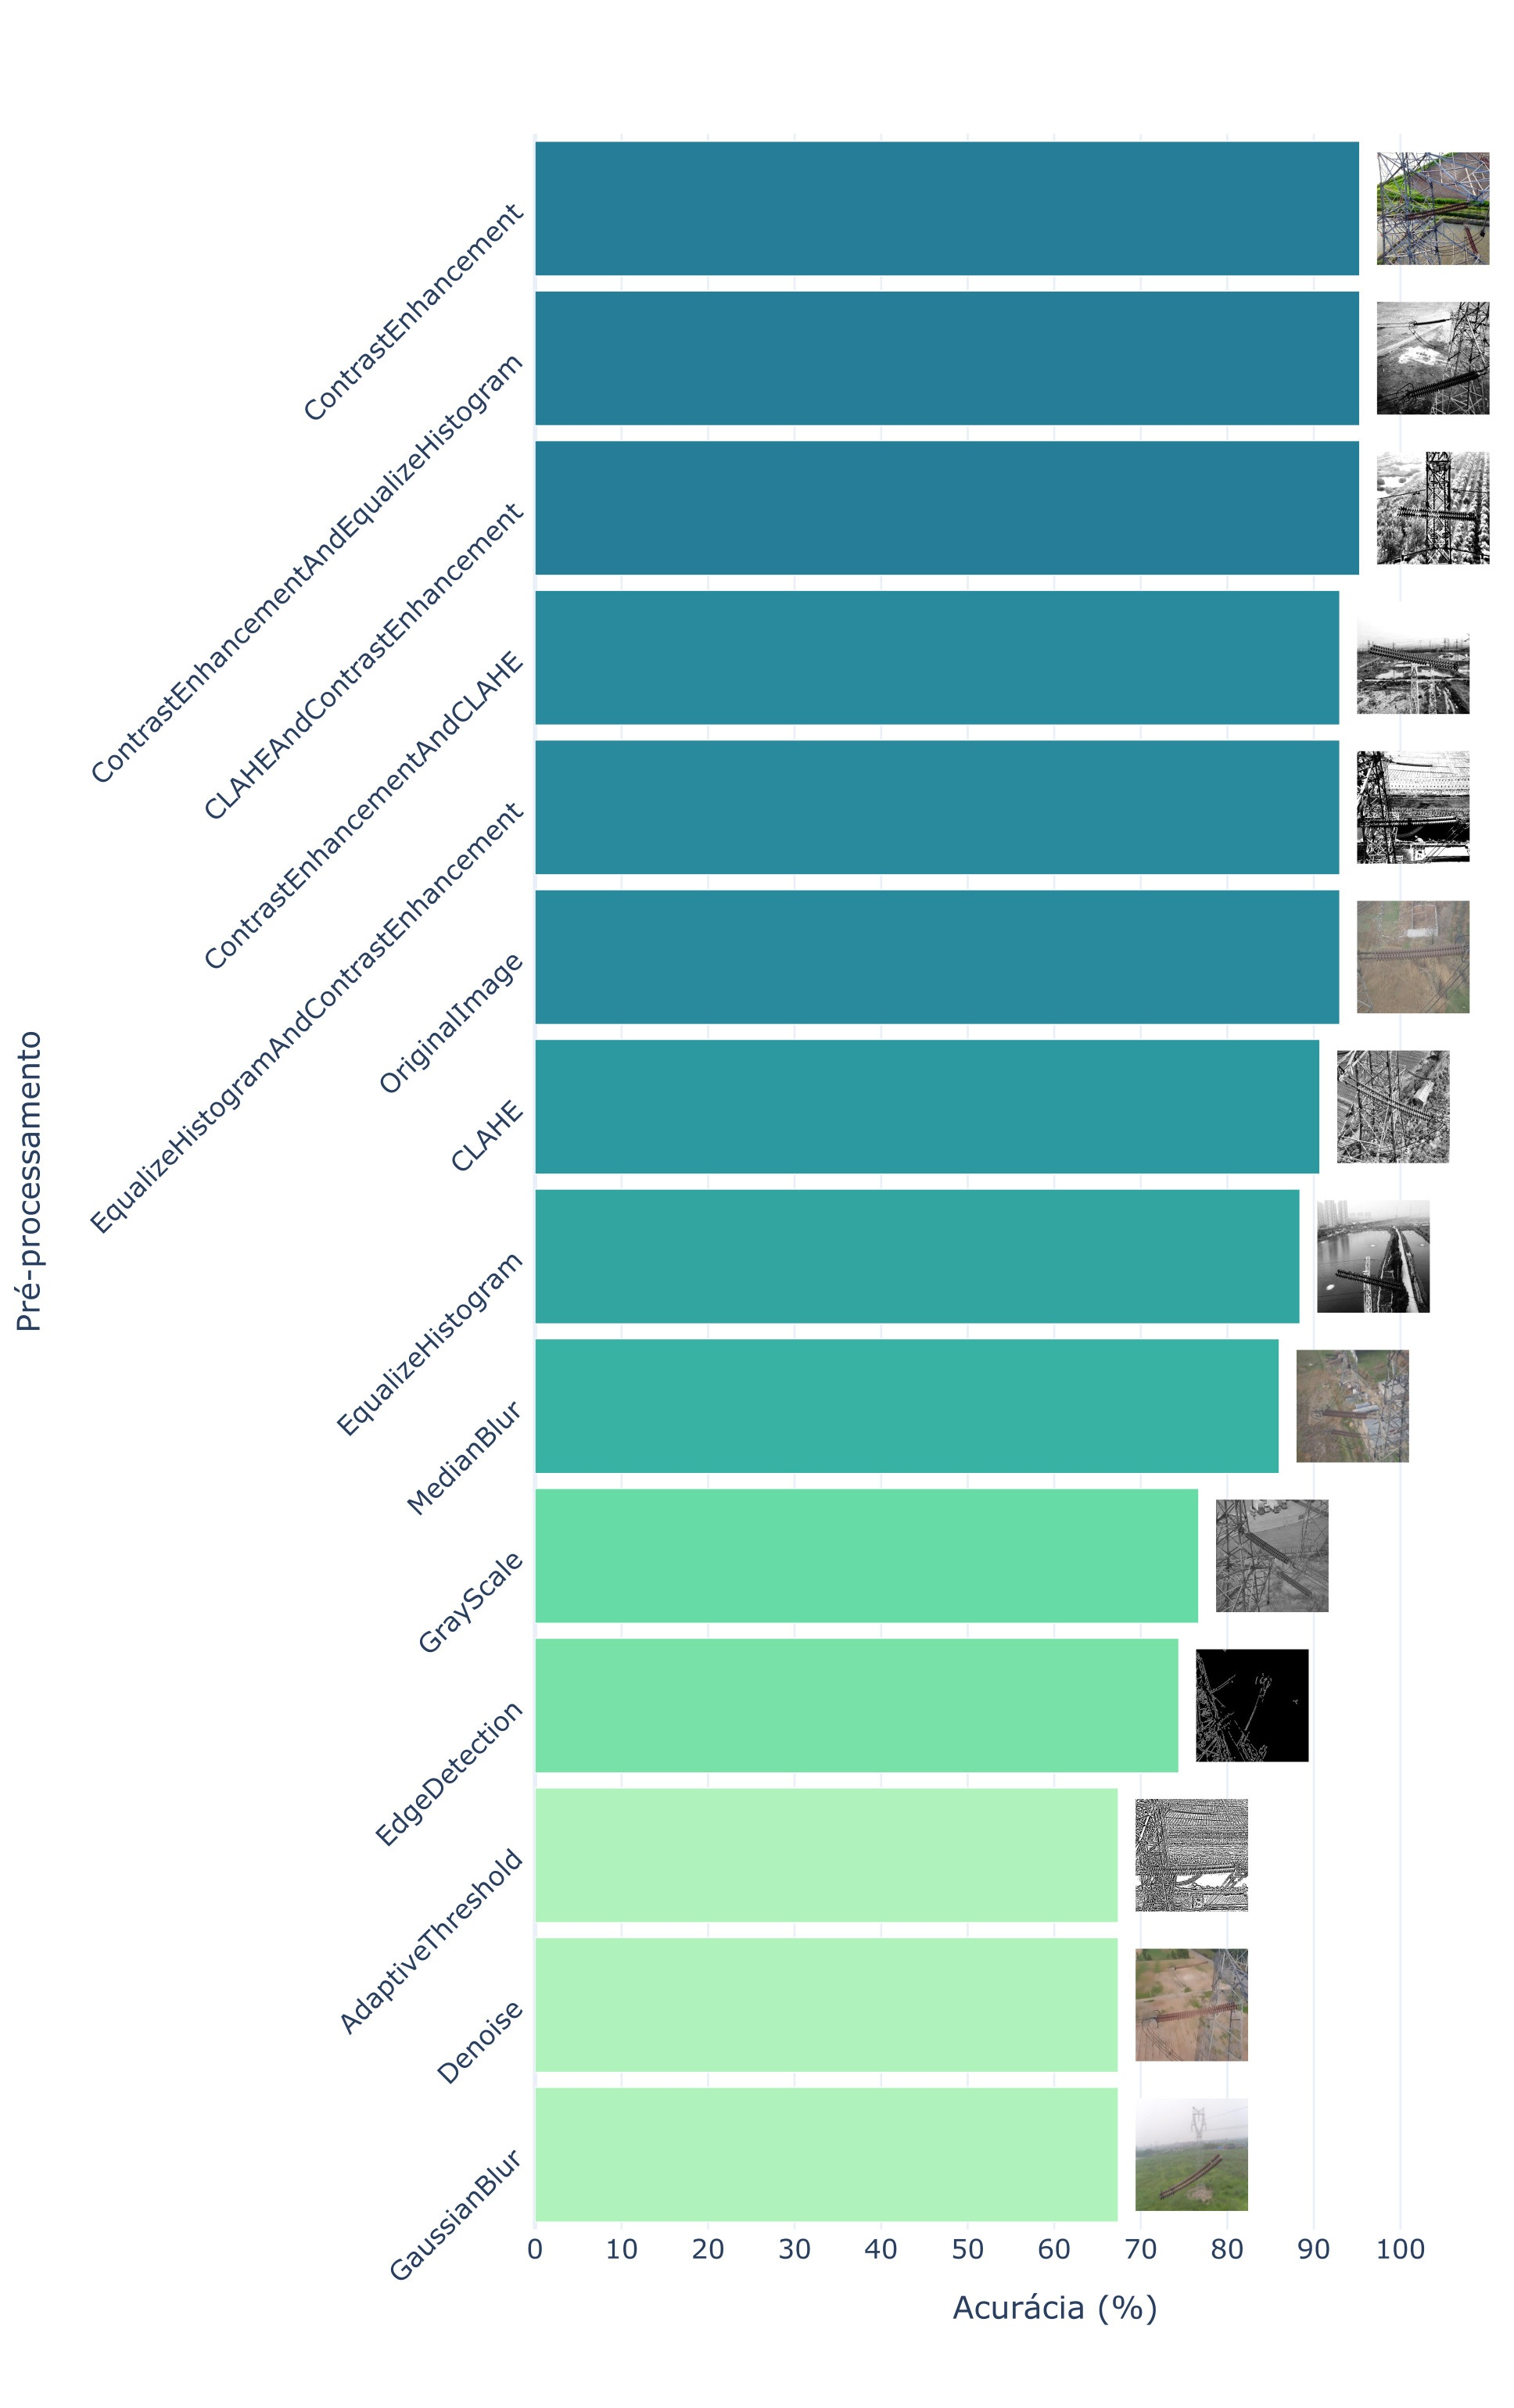
\includegraphics[width=0.46\textwidth]{img/cplid_acc.jpg}
    \caption{Acurácia das diferentes estratégias de pré-processamento avaliadas no \textit{dataset} CPLID.}
    \label{fig:cplid_acc}
\end{figure}

\subsection{Avaliação no \textit{Dataset} DRNPW}

No conjunto de imagens obtidas por drones (DRNPW), a forte presença de fundos com vegetação e estruturas metálicas reduziu a eficácia das técnicas simples que funcionaram bem no CPLID. O melhor resultado veio de uma abordagem híbrida: \textbf{\textit{Contrast Enhancement} seguido de \textit{Equalize Histogram}}. Essa combinação alcançou 83,33\% de acurácia, isolando de forma eficiente os objetos de interesse do fundo ruidoso.

Conversões como a de tons de cinza (\textit{Gray Scale}) não lidaram bem com as variações tonais e compartilham o menor valor observado, 63,33\% de acurácia, o que evidencia a importância da informação de cor para o classificador localizar objetos em cenas ruidosas, comportamento também relatado em estudos que avaliam a sensibilidade de modelos de aprendizado de máquina à supressão de cor e a realces de imagem \cite{chen2023robustness}.

O contraste com o CPLID é o resultado mais relevante desta comparação. Aqui a imagem sem tratamento fica em 63,33\%, abaixo do piso majoritário, e a melhor combinação chega a 83,33\%, ganho de seis acertos em 30 imagens. É neste cenário, de fundo heterogêneo e forte poluição visual, que o pré-processamento produz efeito de magnitude apreciável. A acurácia de todos os métodos aplicados nessa base é apresentada na Fig. \ref{fig:drnpw_acc}.

\begin{figure}[H]
    \centering
    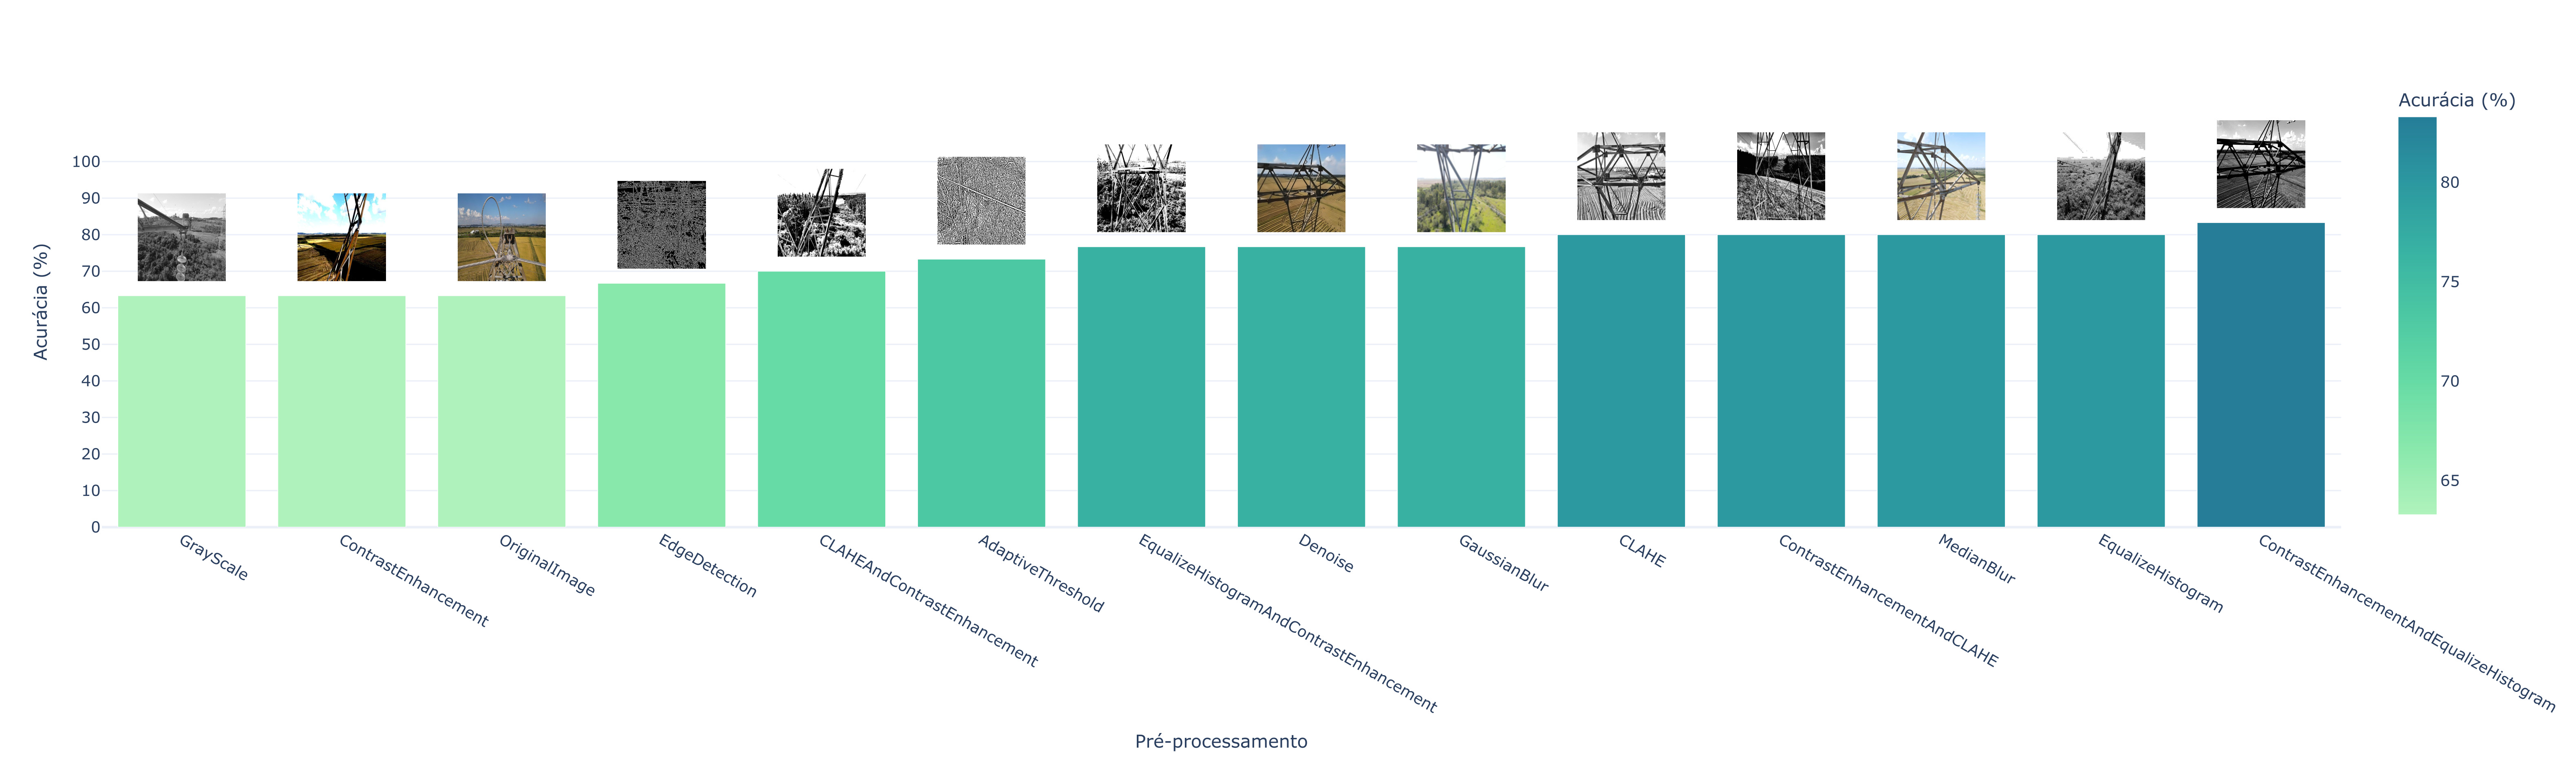
\includegraphics[width=0.46\textwidth]{img/drnpw_acc.jpg}
    \caption{Acurácia das diferentes estratégias de pré-processamento avaliadas no \textit{dataset} DRNPW.}
    \label{fig:drnpw_acc}
\end{figure}

\subsection{Otimização Paramétrica}

Com base nos bons resultados da técnica de ajuste de contraste, adotaram-se duas abordagens de otimização do hiperparâmetro de amplificação (\texttt{factor}), a Busca em Grade (\textit{Grid Search}) e a Busca Aleatória (\textit{Random Search}), ambas conduzidas sobre o DRNPW. Cada valor do fator foi avaliado com um treinamento independente de 5 épocas, o que reduz o custo da varredura e explica a diferença entre os valores absolutos desta subseção e os da avaliação anterior, feita com 50 épocas.

\subsubsection{Busca em Grade (\textit{Grid Search})}

A Busca em Grade foi estruturada em 5 partições lineares. Conforme a Tabela \ref{tab:resultados_grid_search}, o melhor desempenho de validação foi obtido com o fator 1,333, alcançando 90,0\% de acurácia. Fatores muito baixos, como 0,5, resultaram no pior desempenho observado (76,7\%).

\begin{table}[H]
    \centering
    \caption{Resultados da otimização por busca em grade do parâmetro de contraste (\texttt{factor})}
    \label{tab:resultados_grid_search}
    \vspace{0.1cm}
    \begin{tabular}{ccccc}
        \hline
        \textbf{Fator} & \textbf{Acurácia} & \textbf{Precisão} & \textbf{Recall} & \textbf{F1-Score} \\
        \hline
        0,5     & 0,767    & 0,588    & 0,767  & 0,665 \\
        0,778   & 0,833    & 0,694    & 0,833  & 0,758 \\
        1,056   & 0,800    & 0,640    & 0,800  & 0,711 \\
        \textbf{1,333}   & \textbf{0,900}    & \textbf{0,810}    & \textbf{0,900}  & \textbf{0,853} \\
        1,611   & 0,833    & 0,694    & 0,833  & 0,758 \\
        \hline
    \end{tabular}
\end{table}

\subsubsection{Busca Aleatória (\textit{Random Search})}

Para explorar valores intermediários entre as faixas discretas e testar variações extremas, aplicou-se também uma amostragem aleatória, com 5 tentativas em uma distribuição contínua.

De acordo com a Tabela \ref{tab:resultados_random_search}, os resultados confirmaram a sensibilidade do modelo a realces muito intensos (a acurácia caiu para 71,26\% no fator 2,3300). Por outro lado, o melhor resultado ocorreu no fator 1,4364 (85,06\% de acurácia), valor bastante próximo ao encontrado pelo \textit{Grid Search}. As duas buscas confirmam, de forma complementar, que ajustes sutis (próximos de 1,3 e 1,4) são mais eficientes do que realces excessivos.

\begin{table}[H]
    \centering
    \caption{Resultados da otimização estocástica (Random Search) no fator de contraste}
    \label{tab:resultados_random_search}
    \vspace{0.1cm}
    \begin{tabular}{cccc}
        \hline
        \textbf{Tentativa} & \textbf{Fator} & \textbf{Acurácia} & \textbf{Loss (Validação)} \\
        \hline
        1 & \textbf{1,4364} & \textbf{0,8506} & \textbf{4,1418} \\
        2 & 2,8768 & 0,7931 & 4,1455 \\
        3 & 2,3300 & 0,7126 & 4,1499 \\
        4 & 1,9966 & 0,8046 & 4,1416 \\
        5 & 0,8900 & 0,7816 & 4,1480 \\
        \hline
    \end{tabular}
\end{table}

\section{Conclusão}

O trabalho demonstrou que não existe um método de processamento de imagens universal, e que o uso eficiente de Redes Neurais Convolucionais na inspeção de equipamentos elétricos em campo depende de uma escolha criteriosa das técnicas.

Os resultados indicaram que o processamento ideal depende do contexto de fundo da imagem. Em cenários com baixo ruído visual (CPLID), o realce simples de contraste alcançou 95,35\%, valor que supera em um único acerto os 93,02\% da imagem sem tratamento e que, portanto, não caracteriza ganho relevante. Nesse conjunto, a contribuição do método está em descartar transformações destrutivas, como o desfoque gaussiano, que derruba o desempenho para 67,44\%. Já nas imagens aéreas de fundo poluído (DRNPW), combinar equalização global de histograma e ganho de contraste paramétrico elevou a acurácia de 63,33\% para 83,33\%, o único efeito de magnitude apreciável observado neste trabalho. O valor ideal de intensidade, entre 1,3 e 1,4, confirma que realces agressivos são contraproducentes e consolida um fluxo adequado à manutenção automatizada no setor elétrico.

Mais do que os resultados obtidos, a principal contribuição deste trabalho está na própria metodologia. Ao apoiar a escolha das técnicas em indicadores quantitativos (acurácia e \textit{F1-score}) e em uma comparação padronizada entre as abordagens, ela substitui a seleção empírica, baseada em tentativa e erro, por uma avaliação justa e reprodutível. Além disso, a metodologia é expansível, pois novas técnicas podem ser incorporadas e comparadas sob os mesmos critérios. A principal limitação é o tamanho dos conjuntos de teste, de 43 e 30 imagens, em que diferenças de poucos pontos entre técnicas vizinhas situam-se dentro do ruído amostral. A confirmação dos resultados em conjuntos maiores permanece como trabalho futuro.

\begin{thebibliography}{00}
\bibitem{Gonzalez2008} R. C. Gonzalez and R. E. Woods, \textit{Digital Image Processing}, 3rd ed. Upper Saddle River, NJ, USA: Prentice Hall, 2008.

\bibitem{LeCun2015} Y. LeCun, Y. Bengio, and G. Hinton, ``Deep learning,'' \textit{Nature}, vol. 521, no. 7553, pp. 436--444, May 2015, doi: 10.1038/nature14539.

\bibitem{Krizhevsky2012} A. Krizhevsky, I. Sutskever, and G. E. Hinton, ``ImageNet classification with deep convolutional neural networks,'' in \textit{Advances in Neural Information Processing Systems}, vol. 25, 2012, pp. 1097--1105.

\bibitem{Salvi2021} M. Salvi, U. R. Acharya, F. Molinari, and K. M. Meiburger, ``The impact of pre- and post-image processing techniques on deep learning frameworks: A comprehensive review for digital pathology image analysis,'' \textit{Computers in Biology and Medicine}, vol. 128, art. 104129, Jan. 2021, doi: 10.1016/j.compbiomed.2020.104129.

\bibitem{yang2020hyperparameter} L. Yang and A. Shami, ``On hyperparameter optimization of machine learning algorithms: Theory and practice,'' \textit{Neurocomputing}, vol. 415, pp. 295--316, Nov. 2020, doi: 10.1016/j.neucom.2020.07.061.

\bibitem{nguyen2018automatic} V. N. Nguyen, R. Jenssen, and D. Roverso, ``Automatic autonomous vision-based power line inspection: A review of current status and the potential role of deep learning,'' \textit{International Journal of Electrical Power \& Energy Systems}, vol. 99, pp. 107--120, Jul. 2018, doi: 10.1016/j.ijepes.2017.12.016.

\bibitem{wang2023} L. Wang, H. Wan, D. Huang, J. Liu, X. Tang, and L. Gan, ``Sustainable analysis of insulator fault detection based on fine-grained visual optimization,'' \textit{Sustainability}, vol. 15, no. 4, art. 3456, Feb. 2023, doi: 10.3390/su15043456.

\bibitem{eze2022deep} I. Maduako, C. F. Igwe, J. E. Abah, O. E. Onwuasaanya, G. A. Chukwu, F. Ezeji, and F. I. Okeke, ``Deep learning for component fault detection in electricity transmission lines,'' \textit{Journal of Big Data}, vol. 9, no. 1, art. 81, Jun. 2022, doi: 10.1186/s40537-022-00630-2.

\bibitem{sharma2024deep} R. Archana and P. S. E. Jeevaraj, ``Deep learning models for digital image processing: a review,'' \textit{Artificial Intelligence Review}, vol. 57, no. 1, art. 11, Jan. 2024, doi: 10.1007/s10462-023-10631-z.

\bibitem{chen2023robustness} X. Pei, Y. Zhao, L. Chen, Q. Guo, Z. Duan, Y. Pan, and H. Hou, ``Robustness of machine learning to color, size change, normalization, and image enhancement on micrograph datasets with large sample differences,'' \textit{Materials \& Design}, vol. 232, art. 112086, Aug. 2023, doi: 10.1016/j.matdes.2023.112086.

\bibitem{shorten2019survey} C. Shorten and T. M. Khoshgoftaar, ``A survey on image data augmentation for deep learning,'' \textit{Journal of Big Data}, vol. 6, no. 1, art. 60, Jul. 2019, doi: 10.1186/s40537-019-0197-0.

\bibitem{pizer1987adaptive} S. M. Pizer, E. P. Amburn, J. D. Austin, R. Cromartie, A. Geselowitz, T. Greer, B. ter Haar Romeny, J. B. Zimmerman, and K. Zuiderveld, ``Adaptive histogram equalization and its variations,'' \textit{Computer Vision, Graphics, and Image Processing}, vol. 39, no. 3, pp. 355--368, Sep. 1987, doi: 10.1016/S0734-189X(87)80186-X.

\bibitem{ozturk2018histopathological} \c{S}. \"Ozt\"urk and B. Akdemir, ``Effects of histopathological image pre-processing on convolutional neural networks,'' \textit{Procedia Computer Science}, vol. 132, pp. 396--403, 2018, doi: 10.1016/j.procs.2018.05.166.

\bibitem{sciencedirect2023normalization} P. K. Mall, P. K. Singh, S. Srivastav, V. Narayan, M. Paprzycki, T. Jaworska, and M. Ganzha, ``A comprehensive review of deep neural networks for medical image processing: Recent developments and future opportunities,'' \textit{Healthcare Analytics}, vol. 4, art. 100216, Dec. 2023, doi: 10.1016/j.health.2023.100216.

\bibitem{rodrigues2020comparing} L. F. Rodrigues, M. C. Naldi, and J. F. Mari, ``Comparing convolutional neural networks and preprocessing techniques for HEp-2 cell classification in immunofluorescence images,'' \textit{Computers in Biology and Medicine}, vol. 116, art. 103542, Jan. 2020, doi: 10.1016/j.compbiomed.2019.103542.

\bibitem{zhang2022} Z. Zhang, S. Huang, Y. Li, H. Li, and H. Hao, ``Image detection of insulator defects based on morphological processing and deep learning,'' \textit{Energies}, vol. 15, no. 7, art. 2465, Mar. 2022, doi: 10.3390/en15072465.

\bibitem{zheng2022improved} J. Zheng, H. Wu, H. Zhang, Z. Wang, and W. Xu, ``Insulator-defect detection algorithm based on improved YOLOv7,'' \textit{Sensors}, vol. 22, no. 22, art. 8801, Nov. 2022, doi: 10.3390/s22228801.

\bibitem{liu2021} C. Liu, Y. Wu, J. Liu, Z. Sun, and H. Xu, ``Insulator faults detection in aerial images from high-voltage transmission lines based on deep learning model,'' \textit{Applied Sciences}, vol. 11, no. 10, art. 4647, May 2021, doi: 10.3390/app11104647.

\bibitem{he2009learning} H. He and E. A. Garcia, ``Learning from imbalanced data,'' \textit{IEEE Transactions on Knowledge and Data Engineering}, vol. 21, no. 9, pp. 1263--1284, Sep. 2009, doi: 10.1109/TKDE.2008.239.
\end{thebibliography}

\end{document}
